This section will present and interpret the results from the conducted experiments. There are many experimental setups. Three different models evaluated on five datasets with varying amount of compression. Then in addition to that, there is many metrics to be looked at. To illustrate this comprehensive amount of results, Table \ref{tab:comparison} has been constructed. The Table contains the results of three of the five datasets. The Table will be reffered to repeatedly in the following examination of the results. The values that are reffered to is marked with bold.

\subsection{Execution time}
Starting off with looking at the execution time. The training and test time on the synthetic dataset can visually be seen on Figure \ref{fig:performance_time}. It shows no apparent difference between neither the training time or testing of the original and bases model. However, there is a clear difference between those two and DupRes. Both the training in which the uniques are found and in the testing in which the duplicates are looked up adds additional execution time. This performance cost can also clearly be seen in the table for the pendigits dataset. Here we have 93.7/55.3 ms train/test time for the original model, while DupRes with 1 deviation bit has 135/282 ms train/test time. Additionally, it can be seen that DupRes with 6 deviation bits has 145/131 train/test time. This implies that, as the amount of deviation bits rise the testing time decreases. This makes sense as less uniques are found during the training phase, and thus less entries in the table need to be looked through during testing. This incentivize to not use the model if a low amount of duplicates is expected in the data or a low amount of deviation bits is utilized. Originally an implementation utilizing pandas'\cite{pandas} dataframes was used. However, this performed notably worse then the current implementation which uses numpy\cite{numpy} arrays. To optimize this further an implementation could be made in c or c++ and utilize the interoperability to Python.

\begin{figure}
  \centering
  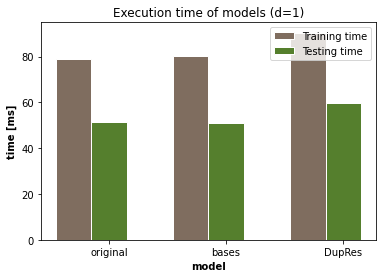
\includegraphics[width=0.8\linewidth]{images/performance_time.png}
  \caption{}
  \label{fig:performance_time}
\end{figure}

\subsection{Metrics and Scoring}
Then we look at the performance of the models in terms of metrics and scoring. Figure \ref{fig:performance_metrics} illustrates the performance metrics of the models on the datasets. In general it can be seen on the figure that the models are performing quite similar. Investigating the metrics for the synthetic dataset a clear pattern can be seen. The bases model performs better than the original, meanwhile DupRes performs better than the bases. The cause of this can be derived from the recall. Since the positives are the inliers the original is simply classifying more inliers as outliers than the others. It is using too few splits in isolating them. As we compress the data the inliers are harder to isolate due to clustering. Utilizing the many duplicates in DupRes we are then classifiying less inliers as outliers. Similar trends is not be seen on the other datasets. On the recall of the pendigit dataset it is seen that the original model predicts less false positives than the others.

Looking at the table there is several interesting observations. All models except two detect every outlier. The two instances are the bases model and DupRes on the synthetic dataset with 6 deviation bits. The bases model predicts every observation as an outlier resulting in 0 scores. Since a lot of data points is grouped with this amount of deviation bits, DupRes will not do the same action as the other model, and therefore have a precision score of 0.98. This implies that one outlier observation might have grouped with the inliers. DupRes will wrongfully push this to be an inlier. Investigating the performance regarding the WBC set it is seen that the performance is almost identical. There are minor discrepancies in the accuracy however the rest is identical. This implies that even though compression is performed, the analytical capabilities is still intact. This is a general trend across all datasets, as was also depicted on Figure \ref{fig:performance_metrics}.

The amount of deviation bits shows a pattern. Looking at the Pendigits dataset the higher the amount of deviation bits the more inliers will be classified as an outlier. This is natural as the compression will place the observations in larger bins that are easier to separate. DupRes does not classify these inliers as outlier as the large binning has resulted in more duplicates and therefore pushing their score towards being an inlier.

\begin{figure}
  \centering
  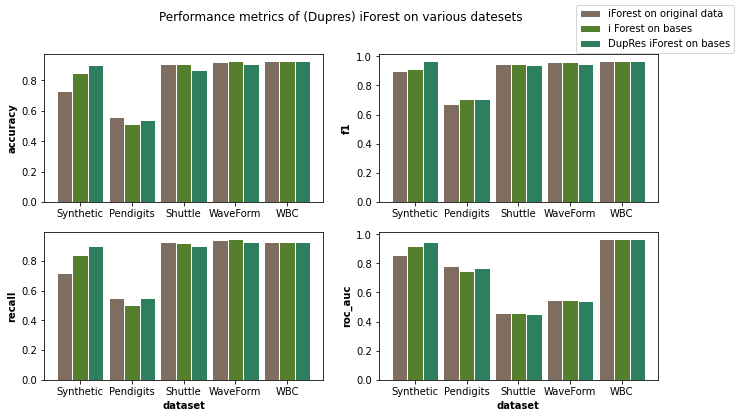
\includegraphics[width=\linewidth]{images/performance_metrics.png}
  \caption{}
  \label{fig:performance_metrics}
\end{figure}
\subsection{Compression and Memory}
The two right-most column in the table describes the compression rate and memory accesed for each model. As the features of all datasets is 8-bit numbers the compression rate is quite simple to calculate: $c_{rate}=\frac{d}{8}$, where $d$ is the amount of deviation bits. The original model naturally has no compression. The two others compression varies on the their amount of deviation bits. $d=6$ for both of the models catches all outliers except on the synthetic data set as described previously. This is a quite significant compression rate of 75\%. Memory Accessed describe how much of the original data that is accesed. It is kind of the reverse of the compression rate. Most interestingly is the DupRes which also has the count table. This is to illustrate that it needs to store the table of uniques and their counts in memory. This shows the tradeoff with DupRes and performing original Isolation Forest on the bases. They have the same compression rate. However, DupRes needs additional memory to store the table. As seen in the results, the training time spent creating the table and the testing time looking up in the table is not to be neglected.       

\begin{table*}[t]
  \centering\sffamily
  \renewcommand{\theadfont}{\normalsize\bfseries}
  \setcellgapes{1ex}\makegapedcells
  \begin{tabular}{*{10}{|c}|c|}
    \hline
    \multirowthead{2}{Model} & \multirowthead{2}{Dataset} & \multirowthead{2}{Dev. bits} & \multicolumn{4}{c|}{\bfseries Metric} & \multicolumn{2}{c|}{\bfseries Time} & \multirowthead{2}{Compression Rate} & \multirowthead{2}{Memory Accessed}                                                                   \\
    \cline{4-9}
                             &                            &                              & \textbf{acc.}                         & \textbf{f1}                         & \textbf{rec.}                       & \textbf{prec.}                     & \textbf{T(ms)} & \textbf{E(ms)} &                               \\
    \hline
    Original                 & Synthetic                  &                              & 0.75                                  & 0.85                                & 0.73                                & 1                                  & 78.8           & 51.4           & 0\%    & 100\%                \\

    \cline{2-11}
                             & Pendigits                  &                              & 0.54                                  & 0.70                                & 0.54                                & 1                                  & \textbf{93.7}  & \textbf{55.3}  & 0\%    & 100\%                \\

    \cline{2-11}
                             & WBC                        &                              & 0.94                                  & 0.97                                & 0.94                                & 1                                  & 75.2           & 22.0           & 0\%    & 100\%                \\
    \hline

    \multirow{9}{*}{Bases}   & \multirow{3}{*}{Synthetic} & 1                            & 0.72                                  & 0.83                                & 0.71                                & 1                                  & 80.2           & 51.2           & 12.5\% & 87.5\%               \\
    \cline{3-11}
                             &                            & 3                            & 0.90                                  & 0.95                                & 0.90                                & 1                                  & 74.6           & 46.4           & 37.5\% & 62.5\%               \\
    \cline{3-11}
                             &                            & 6                            & 0.04                                  & 0                                   & 0                                   & \textbf{0}                         & 74.3           & 45.0           & 75.0\% & 25.0\%               \\
    \cline{2-11}
                             & \multirow{3}{*}{Pendigits} & 1                            & \textbf{0.53}                                  & 0.70                                & 0.53                                & 1                                  & 95.1           & 55.7           & 12.5\% & 87.5\%               \\
    \cline{3-11}
                             &                            & 3                            & \textbf{0.51}                                  & 0.67                                & 0.51                                & 1                                  & 94.3           & 55.9           & 37.5\% & 62.5\%               \\
    \cline{3-11}
                             &                            & 6                            & \textbf{0.42}                                  & 0.59                                & 0.41                                & 1                                  & 95.3           & 56.0           & 75.0\% & 25.0\%               \\
    \cline{2-11}
                             & \multirow{3}{*}{WBC}       & 1                            & 0.94                                  & 0.97                                & 0.94                                & 1                                  & 75.3           & 21.6           & 12.5\% & 87.5\%               \\
    \cline{3-11}
                             &                            & 3                            & 0.94                                  & 0.97                                & 0.94                                & 1                                  & 75.6           & 21.6           & 37.5\% & 62.5\%               \\
    \cline{3-11}
                             &                            & 6                            & 0.95                                  & 0.97                                & 0.94                                & 1                                  & 74.8           & 21.4           & 75.0\% & 25.0\%               \\
    \hline
    \multirow{9}{*}{DupRes}  & \multirow{3}{*}{Synthetic} & 1                            & 0.87                                  & 0.93                                & 0.87                                & 1                                  & 90.4           & 59.7           & 12.5\% & 87.5\% + count table \\
    \cline{3-11}
                             &                            & 3                            & 0.92                                  & 0.95                                & 0.91                                & 1                                  & 85.8           & 55.4           & 37.5\% & 62.5\% + count table \\
    \cline{3-11}
                             &                            & 6                            & 0.98                                  & 0.99                                & 1.00                                & \textbf{0.98}                      & 86.5           & 53.4           & 75.0\% & 25.0\% + count table \\
    \cline{2-11}
                             & \multirow{3}{*}{Pendigits} & 1                            & \textbf{0.54}                                  & 0.70                                & 0.53                                & 1                                  & \textbf{135}   & \textbf{282}   & 12.5\% & 87.5\% + count table \\
    \cline{3-11}
                             &                            & 3                            & \textbf{0.50}                                  & 0.67                                & 0.50                                & 1                                  & 135            & 286            & 37.5\% & 62.5\% + count table \\
    \cline{3-11}
                             &                            & 6                            & \textbf{0.80}                                  & 0.89                                & 0.80                                & 1                                  & \textbf{145}   & \textbf{131}   & 75.0\% & 25.0\% + count table \\
    \cline{2-11}
                             & \multirow{3}{*}{WBC}       & 1                            & 0.94                                  & 0.97                                & 0.94                                & 1                                  & 86.9           & 23.4           & 12.5\% & 87.5\% + count table \\
    \cline{3-11}
                             &                            & 3                            & 0.94                                  & 0.97                                & 0.94                                & 1                                  & 87.7           & 23.7           & 37.5\% & 62.5\% + count table \\
    \cline{3-11}
                             &                            & 6                            & 0.95                                  & 0.97                                & 0.94                                & 1                                  & 85.6           & 23.5           & 75.0\% & 25.0\% + count table \\
    \hline
  \end{tabular}
  \caption{Table of stuff}
  \label{tab:comparison}
\end{table*}